\documentclass{article}\usepackage[]{graphicx}\usepackage[]{xcolor}
% maxwidth is the original width if it is less than linewidth
% otherwise use linewidth (to make sure the graphics do not exceed the margin)
\makeatletter
\def\maxwidth{ %
  \ifdim\Gin@nat@width>\linewidth
    \linewidth
  \else
    \Gin@nat@width
  \fi
}
\makeatother

\definecolor{fgcolor}{rgb}{0.345, 0.345, 0.345}
\newcommand{\hlnum}[1]{\textcolor[rgb]{0.686,0.059,0.569}{#1}}%
\newcommand{\hlsng}[1]{\textcolor[rgb]{0.192,0.494,0.8}{#1}}%
\newcommand{\hlcom}[1]{\textcolor[rgb]{0.678,0.584,0.686}{\textit{#1}}}%
\newcommand{\hlopt}[1]{\textcolor[rgb]{0,0,0}{#1}}%
\newcommand{\hldef}[1]{\textcolor[rgb]{0.345,0.345,0.345}{#1}}%
\newcommand{\hlkwa}[1]{\textcolor[rgb]{0.161,0.373,0.58}{\textbf{#1}}}%
\newcommand{\hlkwb}[1]{\textcolor[rgb]{0.69,0.353,0.396}{#1}}%
\newcommand{\hlkwc}[1]{\textcolor[rgb]{0.333,0.667,0.333}{#1}}%
\newcommand{\hlkwd}[1]{\textcolor[rgb]{0.737,0.353,0.396}{\textbf{#1}}}%
\let\hlipl\hlkwb

\usepackage{framed}
\makeatletter
\newenvironment{kframe}{%
 \def\at@end@of@kframe{}%
 \ifinner\ifhmode%
  \def\at@end@of@kframe{\end{minipage}}%
  \begin{minipage}{\columnwidth}%
 \fi\fi%
 \def\FrameCommand##1{\hskip\@totalleftmargin \hskip-\fboxsep
 \colorbox{shadecolor}{##1}\hskip-\fboxsep
     % There is no \\@totalrightmargin, so:
     \hskip-\linewidth \hskip-\@totalleftmargin \hskip\columnwidth}%
 \MakeFramed {\advance\hsize-\width
   \@totalleftmargin\z@ \linewidth\hsize
   \@setminipage}}%
 {\par\unskip\endMakeFramed%
 \at@end@of@kframe}
\makeatother

\definecolor{shadecolor}{rgb}{.97, .97, .97}
\definecolor{messagecolor}{rgb}{0, 0, 0}
\definecolor{warningcolor}{rgb}{1, 0, 1}
\definecolor{errorcolor}{rgb}{1, 0, 0}
\newenvironment{knitrout}{}{} % an empty environment to be redefined in TeX

\usepackage{alltt}
\usepackage{amsmath} %This allows me to use the align functionality.
                     %If you find yourself trying to replicate
                     %something you found online, ensure you're
                     %loading the necessary packages!
\usepackage{amsfonts}%Math font
\usepackage{graphicx}%For including graphics
\usepackage{hyperref}%For Hyperlinks
\usepackage[shortlabels]{enumitem}% For enumerated lists with labels specified
                                  % We had to run tlmgr_install("enumitem") in R
\hypersetup{colorlinks = true,citecolor=black} %set citations to have black (not green) color
\usepackage{natbib}        %For the bibliography
\setlength{\bibsep}{0pt plus 0.3ex}
\bibliographystyle{apalike}%For the bibliography
\usepackage[margin=0.50in]{geometry}
\usepackage{float}
\usepackage{multicol}

%fix for figures
\usepackage{caption}
\newenvironment{Figure}
  {\par\medskip\noindent\minipage{\linewidth}}
  {\endminipage\par\medskip}
\IfFileExists{upquote.sty}{\usepackage{upquote}}{}
\begin{document}

\vspace{-1in}
\title{Lab 5 -- MATH 240 -- Computational Statistics}

\author{
  Jake Schneider \\
  Colgate University  \\
  Department of Mathematics  \\
  {\tt jdschneider@colgate.edu}
}

\date{2/25/2025}

\maketitle

\begin{multicols}{2}
\begin{abstract}
In this lab, we aim to find out if Manchester Orchestra, The Front Bottoms, or All Get Out contributed the most to a song that they all collaborated on called ``Allentown". In attempt to answer this question we downloaded all releases before ``Allentown" totaling to 180 tracks that we analyze various metrics on. Using these metrics we showcased multiple box plots that indicate to us that Manchester Orchestra had the biggest impact on this collaboration. 


\end{abstract}

\noindent \textbf{Keywords:} Objects; Loops; Libraries; Data Frames

\section{Introduction}
In this lab we start attempting to analyze the contributing influences on the song ``Allentown" by The Front Bottoms, All Get Out and Manchester Orchestra. The 180 songs that we analyzed consisted of all releases before ``Allentown" except for joint albums, live albums, and single releases contained in a full album or an Extended Play. We used Essentia \citep{essentia}, Essentia Models \citep{essentiamodels} and The Lingusitic Inquiry and Word Count/LIWC \citep{LIWC} to aid our analysis of each song. Essentia , an open source musical analysis tool, allowed us do a spectrogram analysis. Essentia Models  was used to collect information about the sound of these songs in human terms (happy, sad, angry, etc.). These different tools allow us to analyze a broader array of the impact that each band might have had.  

After analyzing all 180 songs and ``Allentown" we combined all of the data into one data frame aiming to identify 12 metrics that would help show which band could have had the biggest influence. With these features we created a five number summary which we would use to compare to ``Allentown". 



\section{Methods}
The data that we collected on our 180 songs contained both numerical and categorical variables. The Essentia that we extracted from these songs was contained in \texttt{.JSON} files, while the other two were in \texttt{CSV} files. In order to extract the Essentia \citep{essentia} data from the \texttt{.JSON} files we utilized the stringr package \citep{stringr} and jsonlite package \citep{jsonlite}. Using the {\tt{fromJSON()}} function gave us a large list. Using an empty vector and a \texttt{for} loop allows us to create a data frame with the \texttt{.JSON} file as the row and extract the following variables: overall loudness, spectral energy, dissonance, pitch salience, tempo in beats per minute (bpm), beat loudness, danceability, and tuning frequency. After loading both \texttt{EssentiaModelOutput.csv} and \texttt{LIWCOutput.csv} we now have three data frames of information to work with.  
 

\subsection{Cleaning and Merging \texttt{CSV} File Data}
To tidy up our data in the \texttt{EssentiaModelOutput.csv} we took the averages of the following columns: valence, arousal, happy mood, party mood, relaxed mood, sad mood, acoustic, electric, and instrumental. Keeping these averages we removed every other column except for the artist, album and track. The {\texttt{LIWCOutput.csv}} had information regarding thoughts, feelings and personality traits based on lyrics and we left that \texttt{CSV} file as is.

Using the \verb|merge()| function we were able to merge our original data frame and the two {\texttt{CSV}} files that we downloaded. To ensure that we did not duplicate any rows during this process we set the artist, album and track columns equal to each others which made sure that when the data frames merged we were still left with 181 rows. With all of the information combined we create two new {\texttt{CSV}} files, one with only the song ``Allentown" and one with all the other songs except ``Allentown".

\subsection{Creating Summary Stats}
Using the new \texttt{CSV} file without ``Allentown" we created a five number summary for each band to determine whether ``Allentown" is out of range, unusual or within the range for each band. It is important to note that before creating our five number summary we proceed to keep only the numerical columns in our data frame so that we could compute our five number summary. With all the numerical variables summarized we used the \verb|mutate()| function to create two new columns indicating whether our features value for ``Allentown" was out of range, unusual or within range. We define out of range as being less and the minimum or greater than the maximum, unusual as being between the minimum and the 25 percentile or between the maximum and the 75 percentile and within range if it is within the IQR. 


\subsection{Plotting Data}
After creating the summary stats for each band we then filtered each feature to see whether it was unusual or out of range. The reason for this is because if all three bands are within range on a feature then that is not indicative of much and on the same token if all three bands are out of range then that doesn't tell us much either. However, the reason for filtering this way allowed us to see which band might be in range while the other two bands are out of range for certain features indicating that they might have had more of an influence on that feature. Once filtering this way we searched for features that appeared twice which told us that the third feature had to be in range. This left us with 42 features to choose from. We selected 12 features to create box plots for where we also ploted the value for ``Allentown". 



\section{Results}
To answer our question of which band had the biggest impact on the song ``Allentown" have analyzed 





\section{Discussion}





%%%%%%%%%%%%%%%%%%%%%%%%%%%%%%%%%%%%%%%%%%%%%%%%%%%%%%%%%%%%%%%%%%%%%%%%%%%%%%%%
% Bibliography
%%%%%%%%%%%%%%%%%%%%%%%%%%%%%%%%%%%%%%%%%%%%%%%%%%%%%%%%%%%%%%%%%%%%%%%%%%%%%%%%
\vspace{2em}


\begin{tiny}
\bibliography{bib}
\end{tiny}

\end{multicols}

%%%%%%%%%%%%%%%%%%%%%%%%%%%%%%%%%%%%%%%%%%%%%%%%%%%%%%%%%%%%%%%%%%%%%%%%%%%%%%%%
% Appendix
%%%%%%%%%%%%%%%%%%%%%%%%%%%%%%%%%%%%%%%%%%%%%%%%%%%%%%%%%%%%%%%%%%%%%%%%%%%%%%%%
\section{Appendix}

\begin{center}
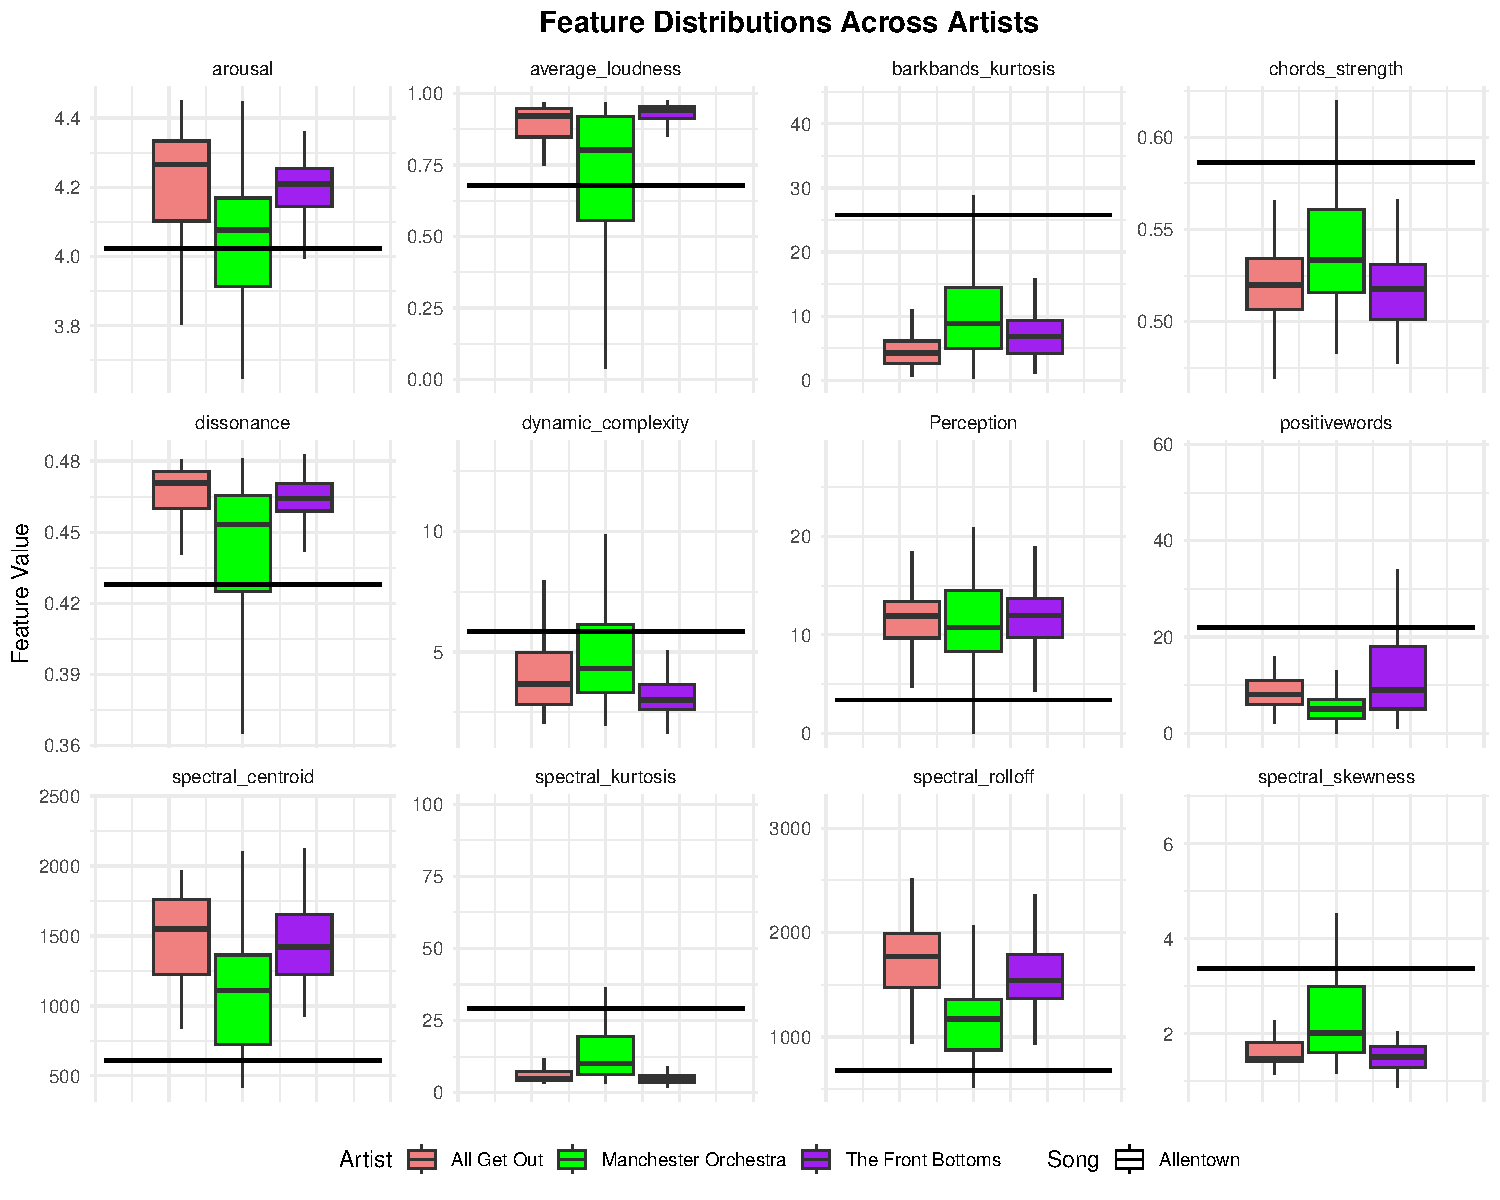
\includegraphics[width=\textwidth]{feature.plot.pdf}  % Include the saved plot
\label{boxplots}
\end{center}



\begin{table}[ht]
\centering
\begin{tabular}{rlrrrrllll}
  \hline
 & artist & min & LF & UF & max & out.of.range & unusual & description & feature \\ 
  \hline
1 & All Get Out & 1.14 & 0.81 & 2.42 & 4.12 & FALSE & TRUE & Outlying & spectral\_skewness \\ 
  2 & Manchester Orchestra & 1.16 & -0.49 & 5.09 & 6.75 & FALSE & FALSE & Within Range & spectral\_skewness \\ 
  3 & The Front Bottoms & 0.87 & 0.63 & 2.40 & 2.04 & TRUE & TRUE & Out Of Range & spectral\_skewness \\ 
  4 & All Get Out & 935.91 & 701.91 & 2767.30 & 2520.04 & TRUE & TRUE & Out Of Range & spectral\_rolloff \\ 
  5 & Manchester Orchestra & 518.87 & 151.27 & 2083.17 & 2566.67 & FALSE & FALSE & Within Range & spectral\_rolloff \\ 
  6 & The Front Bottoms & 927.04 & 740.58 & 2421.46 & 3190.29 & TRUE & TRUE & Out Of Range & spectral\_rolloff \\ 
  7 & All Get Out & 3.03 & -0.36 & 11.90 & 40.10 & FALSE & TRUE & Outlying & spectral\_kurtosis \\ 
  8 & Manchester Orchestra & 3.36 & -13.58 & 39.36 & 98.58 & FALSE & FALSE & Within Range & spectral\_kurtosis \\ 
  9 & The Front Bottoms & 1.89 & 0.00 & 9.55 & 10.47 & TRUE & TRUE & Out Of Range & spectral\_kurtosis \\ 
  10 & All Get Out & 836.21 & 419.54 & 2569.37 & 1967.62 & TRUE & FALSE & Out Of Range & spectral\_centroid \\ 
  11 & Manchester Orchestra & 418.64 & -231.76 & 2322.30 & 2106.83 & FALSE & FALSE & Within Range & spectral\_centroid \\ 
  12 & The Front Bottoms & 924.40 & 584.67 & 2298.03 & 2412.48 & TRUE & FALSE & Out Of Range & spectral\_centroid \\ 
  13 & All Get Out & 2.02 & -0.40 & 8.19 & 7.96 & FALSE & FALSE & Within Range & dynamic\_complexity \\ 
  14 & Manchester Orchestra & 1.96 & -0.90 & 10.34 & 13.21 & FALSE & FALSE & Within Range & dynamic\_complexity \\ 
  15 & The Front Bottoms & 1.63 & 1.00 & 5.26 & 6.50 & FALSE & TRUE & Outlying & dynamic\_complexity \\ 
  16 & All Get Out & 0.40 & 0.44 & 0.50 & 0.48 & FALSE & TRUE & Outlying & dissonance \\ 
  17 & Manchester Orchestra & 0.37 & 0.36 & 0.53 & 0.48 & FALSE & FALSE & Within Range & dissonance \\ 
  18 & The Front Bottoms & 0.43 & 0.44 & 0.49 & 0.48 & TRUE & TRUE & Out Of Range & dissonance \\ 
  19 & All Get Out & 0.62 & -2.65 & 11.38 & 17.68 & TRUE & TRUE & Out Of Range & barkbands\_kurtosis \\ 
  20 & Manchester Orchestra & 0.22 & -9.46 & 28.87 & 43.71 & FALSE & FALSE & Within Range & barkbands\_kurtosis \\ 
  21 & The Front Bottoms & 1.14 & -3.58 & 17.15 & 23.90 & TRUE & TRUE & Out Of Range & barkbands\_kurtosis \\ 
  22 & All Get Out & 0.16 & 0.70 & 1.10 & 0.97 & FALSE & TRUE & Outlying & average\_loudness \\ 
  23 & Manchester Orchestra & 0.00 & 0.01 & 1.46 & 0.97 & FALSE & FALSE & Within Range & average\_loudness \\ 
  24 & The Front Bottoms & 0.55 & 0.85 & 1.02 & 0.98 & FALSE & TRUE & Outlying & average\_loudness \\ 
  25 & All Get Out & 0.47 & 0.47 & 0.58 & 0.59 & FALSE & TRUE & Outlying & chords\_strength \\ 
  26 & Manchester Orchestra & 0.48 & 0.45 & 0.63 & 0.62 & FALSE & FALSE & Within Range & chords\_strength \\ 
  27 & The Front Bottoms & 0.48 & 0.46 & 0.58 & 0.57 & TRUE & TRUE & Out Of Range & chords\_strength \\ 
  28 & All Get Out & 3.80 & 3.76 & 4.68 & 4.45 & FALSE & FALSE & Within Range & arousal \\ 
  29 & Manchester Orchestra & 3.65 & 3.53 & 4.55 & 4.45 & FALSE & FALSE & Within Range & arousal \\ 
  30 & The Front Bottoms & 3.88 & 3.98 & 4.42 & 4.44 & FALSE & FALSE & Within Range & arousal \\ 
  31 & All Get Out & 4.67 & 4.14 & 18.91 & 20.89 & TRUE & TRUE & Out Of Range & Perception \\ 
  32 & Manchester Orchestra & 0.00 & -1.06 & 23.87 & 28.37 & FALSE & FALSE & Within Range & Perception \\ 
  33 & The Front Bottoms & 4.27 & 3.74 & 19.66 & 22.56 & TRUE & TRUE & Out Of Range & Perception \\ 
  34 & All Get Out & 2.00 & -1.50 & 18.50 & 58.00 & FALSE & TRUE & Outlying & positivewords \\ 
  35 & Manchester Orchestra & 0.00 & -3.00 & 13.00 & 27.00 & FALSE & TRUE & Outlying & positivewords \\ 
  36 & The Front Bottoms & 1.00 & -14.50 & 37.50 & 34.00 & FALSE & FALSE & Within Range & positivewords \\ 
   \hline
\end{tabular}
\caption{Five Number Summary of Selected Features} 
\label{compared.features}
\end{table}



\onecolumn






\end{document}
